%----------------------------------------------------------------------------------------
%	PACKAGES AND THEMES
%----------------------------------------------------------------------------------------

\documentclass{beamer}
\mode<presentation> {
	\usetheme{Warsaw}
	\setbeamercolor{page_num_color}{fg=white,bg=blue}

	\defbeamertemplate*{footline}{shadow theme}{%
		\leavevmode%
		\hbox{\begin{beamercolorbox}[wd=.5\paperwidth,ht=2.5ex,dp=1.125ex,leftskip=.3cm plus1fil,rightskip=.3cm]{author in head/foot}%
		    \usebeamerfont{author in head/foot}\hfill\insertshortauthor
		\end{beamercolorbox}%
		\begin{beamercolorbox}[wd=.4\paperwidth,ht=2.5ex,dp=1.125ex,leftskip=.3cm,rightskip=.3cm plus1fil]{title in head/foot}%
		    \usebeamerfont{title in head/foot}\insertshorttitle\hfill%
		\end{beamercolorbox}%
		\begin{beamercolorbox}[wd=.1\paperwidth,ht=2.5ex,dp=1.125ex,leftskip=.3cm,rightskip=.3cm plus1fil]{author in head/foot}%
		\hfill\insertframenumber\,/\,\inserttotalframenumber
		\end{beamercolorbox}}%
		\vskip0pt%
	}
}

\usepackage{amsmath}
\usepackage{amssymb}
\usepackage{graphicx} % Allows including images
\usepackage{booktabs} % Allows the use of \toprule, \midrule and \bottomrule in tables
\usepackage[english]{babel}
\usepackage{graphicx}
\usepackage{listings, lstautogobble}
\usepackage{color}
\usepackage{caption}
\usepackage{verbatim}
\usepackage{hyperref}


%----------------------------------------------------------------------------------------
%	LSTSETTING
%----------------------------------------------------------------------------------------
\lstset{language=C,
    keywordstyle=\color{blue}, 
    morekeywords={then},
    numberstyle=\footnotesize,
    basicstyle=\ttfamily\footnotesize,
    numbers=left,
    stepnumber=1,
    frame=single,
    breaklines=true,
    tabsize=4,
    escapeinside={(*}{*)},
    autogobble=true
}

%----------------------------------------------------------------------------------------
%   TITLE PAGE 
%----------------------------------------------------------------------------------------

\title[Collision Detection in VR]
{Collision Detection in VR} % The short title appears at the bottom of every slide, the full title is only on the title page
\author[Yi-Ning Chang \& Ming-Jing Lin]
{   Yi-Ning Chang \& Ming-Jing Lin
} % Your name
\institute[] % Your institution as it will appear on the bottom of every slide, may be shorthand to save space
{
	NTUCSIE \\ % Your institution for the title page
	Parallel and Distributed Processing Laboratory
}
\date{February 22, 2017} % Date, can be changed to a custom date

\begin{document}

%----------------------------------------------------------------------------------------
%	TITLE PAGE SETTING
%----------------------------------------------------------------------------------------
\begin{frame}[noframenumbering]
    \titlepage % Print the title page as the first slide
\end{frame}

\AtBeginSection[]
  {
  	 \setbeamertemplate{footline}{} 
     \begin{frame}<beamer>[noframenumbering]
     \tableofcontents[currentsection, hideallsubsections]
     \end{frame}
     \setbeamertemplate{footline}{%
		\leavevmode%
		\hbox{\begin{beamercolorbox}[wd=.5\paperwidth,ht=2.5ex,dp=1.125ex,leftskip=.3cm plus1fil,rightskip=.3cm]{author in head/foot}%
		    \usebeamerfont{author in head/foot}\hfill\insertshortauthor
		\end{beamercolorbox}%
		\begin{beamercolorbox}[wd=.4\paperwidth,ht=2.5ex,dp=1.125ex,leftskip=.3cm,rightskip=.3cm plus1fil]{title in head/foot}%
		    \usebeamerfont{title in head/foot}\insertshorttitle\hfill%
		\end{beamercolorbox}%
		\begin{beamercolorbox}[wd=.1\paperwidth,ht=2.5ex,dp=1.125ex,leftskip=.3cm,rightskip=.3cm plus1fil]{author in head/foot}%
		\hfill\insertframenumber\,/\,\inserttotalframenumber
		\end{beamercolorbox}}%
		\vskip0pt%
	}
  }


%------------------------------------------------
% Outline
%------------------------------------------------
\begin{frame}
\frametitle{Outline} % Table of contents slide, comment this block out to remove it
\tableofcontents[hideallsubsections] % Throughout your presentation, if you choose to use \section{} and \subsection{} commands, these will automatically be printed on this slide as an overview of your presentation
\end{frame}


%------------------------------------------------
% Introduction
%------------------------------------------------
\section{Introduction}

% Motivation
\subsection{Motivation}
	\begin{frame}
	\frametitle{Motivation}
	\begin{itemize}
		\item Collision detection is one of the critical technique in improving the user experience in VR.
            \begin{itemize}
                \item Collision between the users and the objects.
            \end{itemize}
		\medskip
		\item An user should receive feedbacks while the avatar touches the objects or other users.
            \begin{itemize}
                \item   Be blocked, vibration or the vision feedback.
            \end{itemize}
	\end{itemize}
	\end{frame}

% Current Status
\subsection{Current Status}
	\begin{frame}
	\frametitle{Current Status}
	\begin{itemize}
		\item Online 3D games
			\begin{itemize}
				\item Some MMORPGs don't handle the collisions between users.
				\item Others wraps the characters in cubic or sphere bounds, which makes collision detection much easier.
			\end{itemize}
		\medskip
		\item VR Application
			\begin{itemize}
				\item An user interacts with objects using the controllers.
				\item Real-time human-avatar interaction increases the complexity of multiplayer VR application.
			\end{itemize}
	\end{itemize}
	\end{frame}

% Project Goal
\subsection{Project Goal}
	\begin{frame}
	\frametitle{Project Goal}
	\begin{itemize}
		\item Evaluate the amount of resources required to perform collision detection between user avatars in a social VR application on cloud server.
	\end{itemize}
	\end{frame}

%------------------------------------------------
% Work Items
%------------------------------------------------
\section{Work Items}

% Server
\subsection{Server}
	\begin{frame}
	\frametitle{Server}
	\begin{itemize}
		\item Set up the server.
		\item Receive sensor data from clients.
		\item Perform collision detection.
		\item Monitor the usage of each resource.
	\end{itemize}
	\end{frame}

% Client
\subsection{Client}
	\begin{frame}
	\frametitle{Client}
	\begin{itemize}
		\item Send data to server: position, orientation and body information.
			\begin{itemize}
				\item Two or three real users demonstrate the collision effect by keyboard and screen.
				\item Lots of artificial users to test the scalibility.
				\item Every user has artificial parts with random path, like arms or legs.
			\end{itemize}
		\item Receive information from server.
			\begin{itemize}
				\item The information of other users and objects.
				\item Collision detection.
			\end{itemize}
		\item Display
	\end{itemize}
	\end{frame}

% Evaluation
\subsection{Evaluation}
	\begin{frame}
	\frametitle{Evaluation}
	\begin{itemize}
		\item System scalibility
			\begin{itemize}
				\item Increase the complexity of bounds on avatars and the number of users in limited resources.
				\item Resource management.
			\end{itemize}
		\item System stability
			\begin{itemize}
				\item Correctness
				\item Time consumed.
			\end{itemize}
	\end{itemize}
	\end{frame}

% Expected Deliverables
\subsection{Expected Deliverables}
	\begin{frame}
	\frametitle{Expected Deliverables}
	\begin{itemize}
		\item A better collision detection algorithm in parallel and distributed system.
		\item A resource management system
		\item A simple application with GUI by Unity 3D.
		\item Experimental data.
		\begin{itemize}
			\item eg. resource usage
		\end{itemize}
	\end{itemize}
	\end{frame}

% Gantt chart
\subsection{Gantt Chart}
	\begin{frame}
	\frametitle{Gantt Chart}
	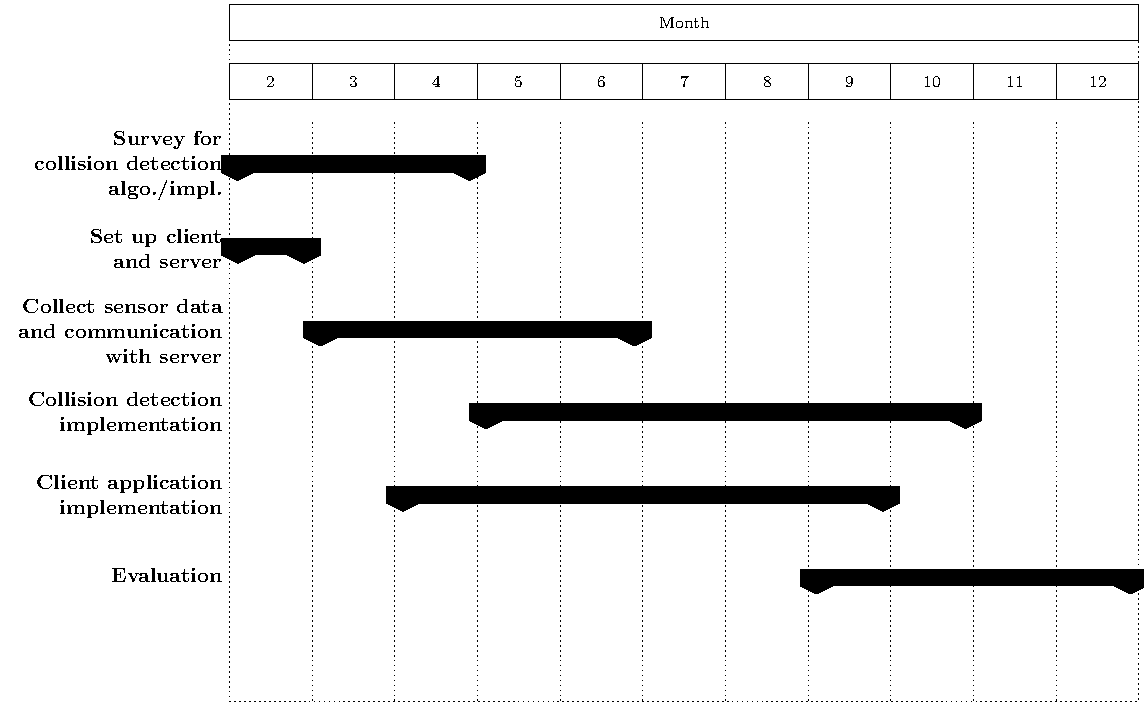
\includegraphics[scale=0.5]{figure/GanttChart.pdf}	
	\end{frame}

%------------------------------------------------
% Reference
%------------------------------------------------
\section{Reference}

% Paper
\subsection{Paper}
	\begin{frame}
	\frametitle{Paper}
	\begin{itemize}
		\item Perfomance comparison between state-of-the-art point-cloud based collision detection approached on the CPU and GPU
			\begin{itemize}
				\item from \it{IFAC-PapersOnline}
			\end{itemize}
		\item Collision detection between point clouds using an efficient k-d tree implementation
			\begin{itemize}
				\item from \it{Advanced Engineering Informatics}
			\end{itemize}
		\item Real-time KD-Tree construction on graphics hardware
			\begin{itemize}
				\item from \it{ACM Advanced Materials Research}
			\end{itemize}
		\item Self-Customized BSP trees for collision detection
			\begin{itemize}
				\item from \it{Computational Geometry}
			\end{itemize}
		\item Unified GPU voxel collision detection for mobile manipulation planning
			\begin{itemize}
				\item from \it{Intelligent Robots and Systems}
			\end{itemize}
	\end{itemize}
	\end{frame}

% Code
\subsection{Code}
	\begin{frame}
	\frametitle{Code}
	\begin{itemize}
		\item Algorithms in Game Engine \href{http://www.haroldserrano.com/blog/algorithms-in-game-engine-development}{Development}
		\item HMD Initialization and Sensor Enumeration Documentation
			\begin{itemize}
				\item from \href{https://developer3.oculus.com/documentation/pcsdk/latest/concepts/dg-sensor/}{Oculus.com}
			\end{itemize}
		\item Collision Detection from \it{jeffThompson} on \href{https://github.com/jeffThompson/CollisionDetection}{GitHub}
		\item JS Game Development - 3D AABB collisions on \href{https://github.com/mozdevs/gamedev-js-3d-aabb}{GitHub}
	\end{itemize}
	\end{frame}

\end{document} 
